\documentclass{article}
\usepackage[utf8]{inputenc}
\usepackage[spanish]{babel}
\usepackage{graphicx}
\usepackage{listings}
\usepackage[autostyle]{csquotes}
\usepackage{float}
\usepackage{fancyhdr}
\pagestyle{fancy}
\rhead{Manuel Ignacio Porto\\96587}
\setlength{\headheight}{23pt}
\begin{document}

\section{Comenzando}

\textbf{¿Qué es Valgrind?}\newline
   
   Valgrind es un framework orientado al desarrollo de herramientas de análisis dinámico que ayudan a la depuracion de problemas de memoria y rendimiento de programas. Una de las herramientas mas usadas es ``Memcheck'' que ofrece detección automática de errores en el manejo de memoria.
    
    \begin{figure}[H]
        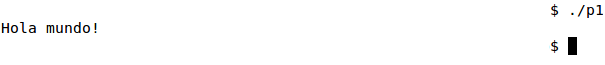
\includegraphics[width=\columnwidth]{p1_svalgrind}
        \caption{Ejecución de aplicativo sin Valgrind}
    \end{figure}
    
     \begin{figure}[H]
        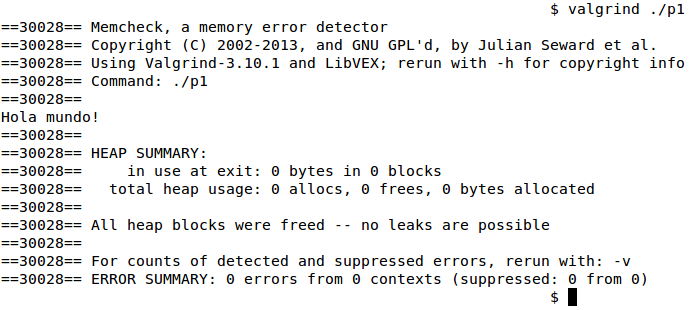
\includegraphics[width=\columnwidth]{p1_valgrind}
        \caption{Ejecución de aplicativo con Valgrind}
    \end{figure}
    
\textbf{¿Qué representa \texttt{sizeof()}? ¿Cuál sería el valor de salida de \texttt{sizeof(char)} y \texttt{sizeof(int)}?}\newline
    
    El operador \texttt{sizeof()} devuelve el tamaño, en bytes, del operando. El valor de retorno de \texttt{sizeof(char)} es siempre 1 byte por definición. El valor de salida de \texttt{sizeof(int)} depende del compilador. Como mínimo debe ser de 2 bytes. En el computador en donde se ejecuto la aplicación, el \texttt{int} posee un tamaño de 4 bytes. \newline

\textbf{``El sizeof() de una struct de C es igual a la suma del sizeof() de cada uno de los elementos de la misma''. Explique la validez o invalidez de dicha afirmación.}\newline

    La afirmación no es válida ya que no toma en cuenta el padding agregado con el fin de cumplir con la condición de alineamiento de un programa. Dicha condición consiste en limitar a todas los tipos de datos a ``ocupar'' un mismo espacio en memoria, esto se logra descartartando los bytes no utilizados y así evitar que otra variable utilice dichos bytes. A continuación se presenta un ejemplo:
    
    \begin{lstlisting}[language=C]
    struct Ejemplo {
    short a; // 2 bytes
             // 2 bytes de padding
    int   b; // 4 bytes
    char  c; // 1 byte
             // 3 bytes de padding
             // Total: 12 bytes
    };
    \end{lstlisting}
    
\section{SERCOM - Error de compilación}
    
\textbf{Documentar el/los error/es reportado/s por SERCOM, utilizando capturas de pantalla.}
    \begin{figure}[H]
        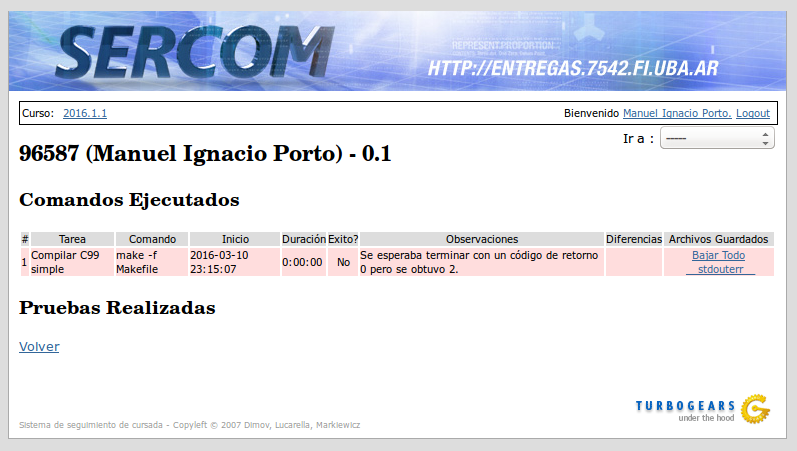
\includegraphics[width=\columnwidth]{p2}
        \caption{Resultado de la entrega}
    \end{figure}
    
    \begin{figure}[H]
        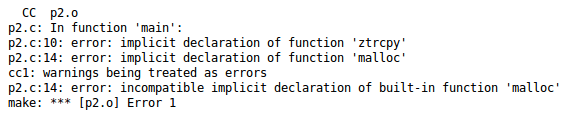
\includegraphics[width=\columnwidth]{p2_stderr}
        \caption{Salida \texttt{\_\_stdouterr\_\_}}
    \end{figure}
    
\textbf{Explicar los errores reportados. ¿Fueron errores del compilador o del linker?}\newline

    Los errores reportados por SERCOM pertenecen al linker. Los errores son causados al hacer referencia a funciones que no están definidas en el código fuente ni en las librerías incluidas. Si bien el compilador lanza una advertencia sobre la declaración implícita de las funciones puede compilar el código, pero al intentar linkear los distintos archivos involucrados el linker no encuentra referencias a las funciones \texttt{ztrncpy} y \texttt{malloc} por lo que lanza un error.
    
\section{SERCOM - Normas de programación y código de salida}
    
\textbf{Captura de pantalla indicando la correcta generación del ejecutable.}
    \begin{figure}[H]
        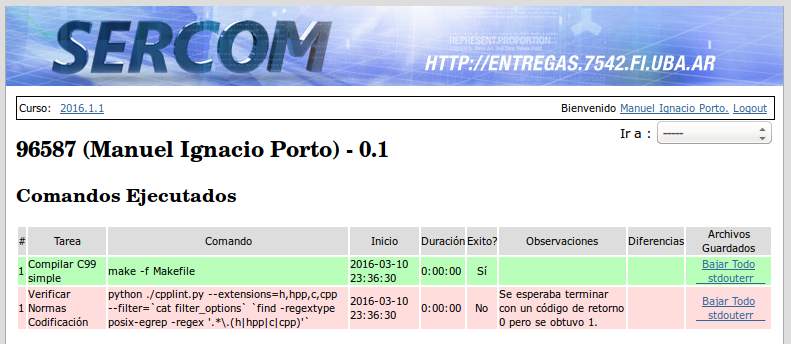
\includegraphics[width=\columnwidth]{p3_compile}
        \caption{Generación correcta del ejecutable}
    \end{figure}

\textbf{Captura de pantalla mostrando los problemas de estilo detectados. Explicar.}    
    \begin{figure}[H]
        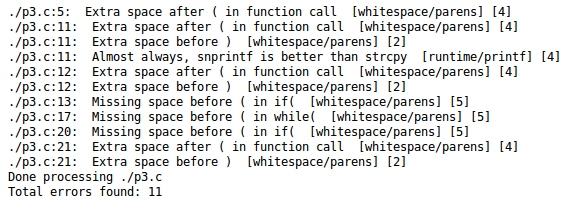
\includegraphics[width=\columnwidth]{p3_style}
        \caption{Problemas de estilo detectados}
    \end{figure}
    
    Los errores de estilo detectados corresponden, en su mayoría, a cantidad espacios faltantes o excesivos luego de declaraciones y llamadas a funciones. También se notifica de un error, en el que se informa que utilizar la función \texttt{snprintf} es mas conveniente y seguro que usar \texttt{strcpy}.\newline

\textbf{Captura de pantalla indicando el error reportado en la prueba 1. Explicar.}    
    
    \begin{figure}[H]
        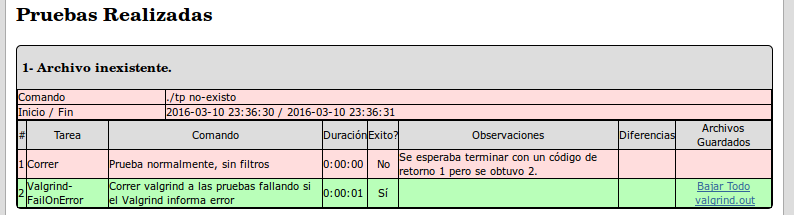
\includegraphics[width=\columnwidth]{p3_test1}
        \caption{Resultados de la prueba 1}
    \end{figure}
        
    \begin{figure}[H]
        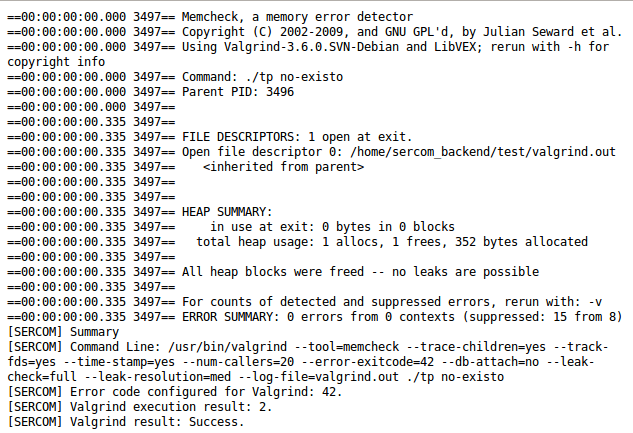
\includegraphics[width=\columnwidth]{p3_valgrind}
        \caption{Salida Valgrind}
    \end{figure}

    El error reportado en la prueba 1 corresponde, al valor de retorno del programa cuando es ejecutado con el nombre de un archivo inexistente como parámetro. En el caso de que esto ocurriese, el aplicativo debería devolver 1 pero devuelve 2. La linea ``\texttt{if( fp == NULL ) return 2;}'' es la causante el problema.

\section{SERCOM - Pérdida de memoria}

\textbf{Captura de pantalla indicando la nueva salida del chequeo de normas de codificación.}
    \begin{figure}[H]
        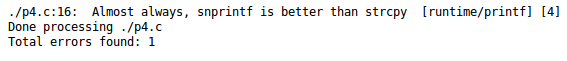
\includegraphics[width=\columnwidth]{p4_style}
        \caption{Salida del chequeo de normas de codificación}
    \end{figure}
    
\textbf{Captura de pantalla indicando la correcta finalización de la prueba 1.}
    \begin{figure}[H]
        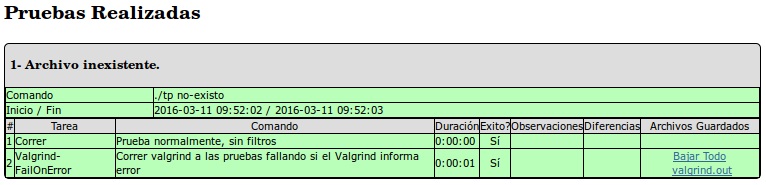
\includegraphics[width=\columnwidth]{p4_test1}
        \caption{Resultados de la prueba 1}
    \end{figure}

\textbf{Captura de pantalla indicando los problemas reportados por Valgrind. Explicar en detalle.}   
    \begin{figure}[H]
        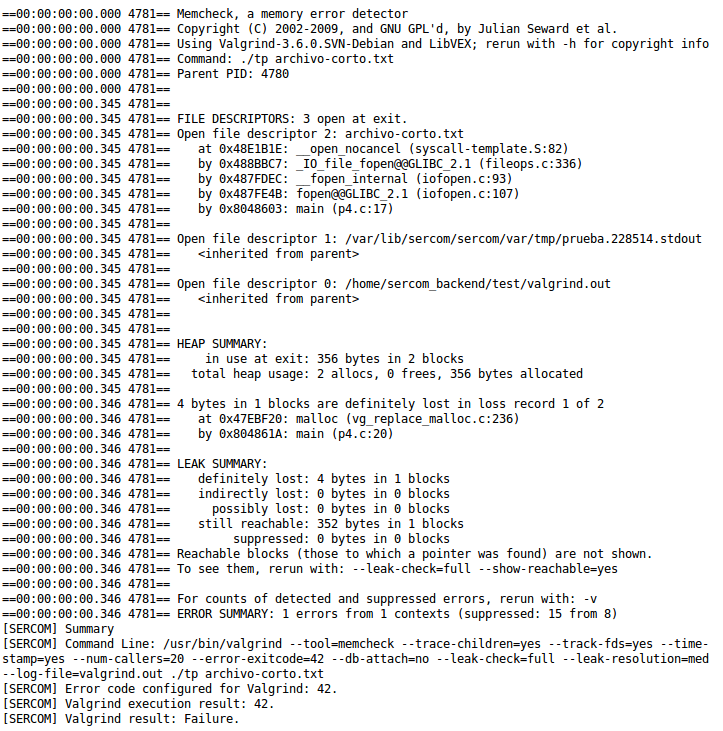
\includegraphics[width=\columnwidth]{p4_valgrind}
        \caption{Problemas reportados por Valgrind}
    \end{figure}
    
    Los errores reportados por Valgrind advierten que un archivo fue abierto (\texttt{fopen}) pero nunca cerrado (\texttt{fclose}) y que se reservó espacio en memoria (\texttt{malloc}) pero que nunca fue liberada, ya que nunca se realizo la operación correspondiente para liberarla (\texttt{free}). Esto produce como consecuencia, que los bytes de memoria reservados se pierdan y que el programa tenga leaks de memoria.

\section{SERCOM - Escrituras fuera de rango}

\textbf{Captura de pantalla de la salida de Valgrind sobre la prueba 2.}

    \begin{figure}[H]
        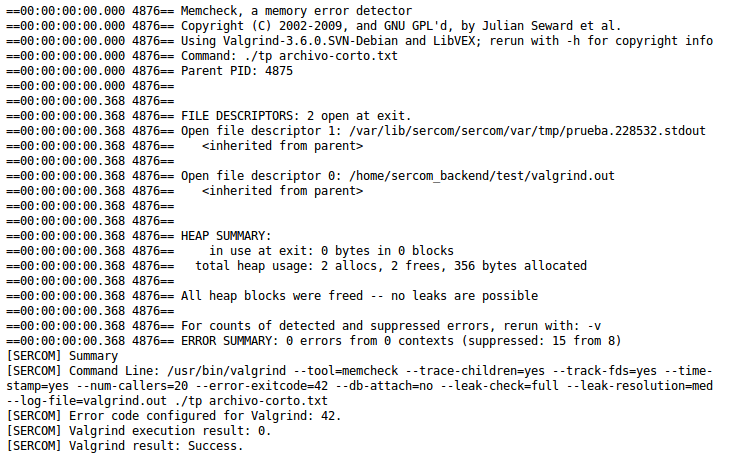
\includegraphics[width=\columnwidth]{p5_valgrind}
        \caption{Salida Valgrind}
    \end{figure}
    
\textbf{Explicar en detalle el problema reportado. ¿Podría solucionarse utilizando \texttt{strncpy} en lugar de
\texttt{strcpy}? ¿Podría ayudar Valgrind a su diagnóstico? (captura de pantalla del mismo).}

    \begin{figure}[H]
        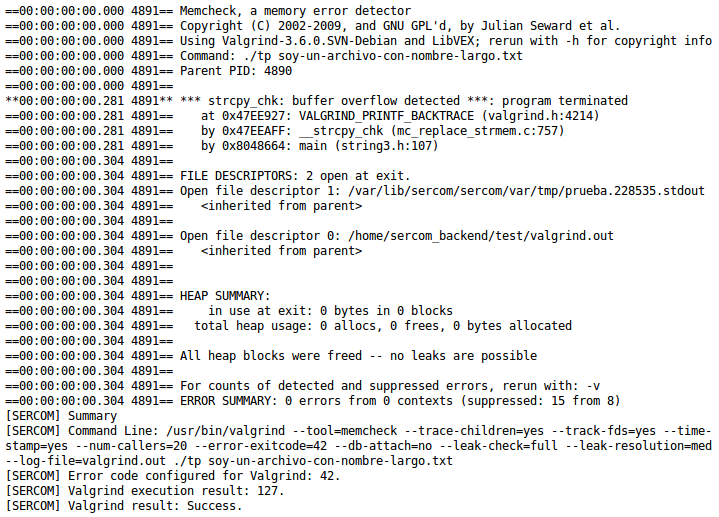
\includegraphics[width=\columnwidth]{p5_valgrind2}
        \caption{Errores reportados por Valgrind}
    \end{figure}
    
    El problema reportado surge al enviar como argumento del aplicativo un nombre de archivo, cuyo largo es mayor que el espacio reservado para almacenar dicho nombre. Al utilizar la función \texttt{strcpy} el programa no posee protección contra un potencial \textit{buffer overflow}, esto es debido a que la mencionada función copia caracteres hasta encontrar un \texttt{'\textbackslash 0'} y no toma en cuenta el largo del buffer en donde se esta copiando la cadena. Por otro lado, utilizando \texttt{strncpy} se especifica una cantidad máxima de caracteres a copiar.
    
    Valgrind ayuda a diagnosticar el error ya que lo informa de manera explicita en su análisis.\newline
    
\textbf{Explicar de qué se trata un \textit{segmentation fault} y un \textit{buffer overflow}.}\newline

    Un \textit{segmentation fault} es error causado por intentar acceder a una posición de memoria invalida, ya sea porque no le pertenece al programa (nunca la reservó o ya la liberó), es de solo lectura, etc. Su propósito es evitar la corrupción de memoria y la introducción de bugs difíciles de encontrar.  
    
    Un \textit{buffer overflow} es una situación generada cuando un programa intenta ingresar mas información que la que un buffer puede almacenar. Un buffer es una sección de memoria contigua y cuando se escribe información fuera de ese rango, el programa puede corromperse exponiéndolo no solo a una finalización inesperada y errónea si no también a la inyección de código malicioso.\newline
    
\textbf{Indicar el contenido de los archivos de entrada utilizados en las pruebas 2 y 4.}

\begin{itemize}
    \item \textbf{Prueba 2}
    
    \blockquote{La estructura de estos cuentos (y de todos los relativos a Holmes) es 
similar: Sherlock está en su casa de Baker Street, muchas veces en compañía 
de su amigo, cuando de repente aparece un personaje que viene a plantearle 
un problema para el que necesita ayuda. Otras veces esta noticia llega a él 
a través del periódico. Los casos son resueltospor la lógica y el 
razonamiento del famoso detective. Son cuentos de misterio, donde interviene 
la intriga y la aventura, unido al análisis psicológico de sus personajes.}

    \item \textbf{Prueba 4}
    
    \blockquote{Rene Geronimo Favaloro (La Plata, Argentina, 12 de julio de 1923 - Buenos 
Aires, Argentina, 29 de julio de 2000) fue un prestigioso medico cirujano 
toracico argentino, reconocido mundialmente por ser quien realizo el primer 
bypass cardiaco en el mundo. Estudio medicina en la Universidad de La Plata 
y una vez recibido, previo paso por el Hospital Policlinico, se mudo a la 
localidad de Jacinto Arauz para reemplazar temporalmente al medico local, 
quien tenia problemas de salud. A su vez, leia bibliografia medica 
actualizada y empezo a tener interes en la cirugia toracica. A fines de la 
decada de 1960 empezo a estudiar una tecnica para utilizar la vena safena 
en la cirugia coronaria. A principios de la decada de 1970 fundo la 
fundacion que lleva su nombre. Se desempeno en la Conadep, condujo 
programas de television dedicados a la medicina y escribio libros. 
Durante la crisis del 2000, su fundacion tenia una gran deuda economica y 
le solicito ayuda al gobierno sin recibir respuesta, lo que lo indujo a 
suicidarse. El 29 de julio de 2000, despues de escribir una carta al 
Presidente De la Rua criticando al sistema de salud, se quito la vida de un 
disparo al corazon.}
\end{itemize}

\textbf{Indicar la línea de comandos utilizada para la ejecución de la prueba 3.}\newline

La linea de comandos utilizada para la ejecución de la prueba 3 es, 

\texttt{./tp soy-un-archivo-con-nombre-largo.txt}.

\section{SERCOM - Entrada estándar}

\textbf{Captura de pantalla con la correcta salida del chequeo de normas de codificación.}

    \begin{figure}[H]
        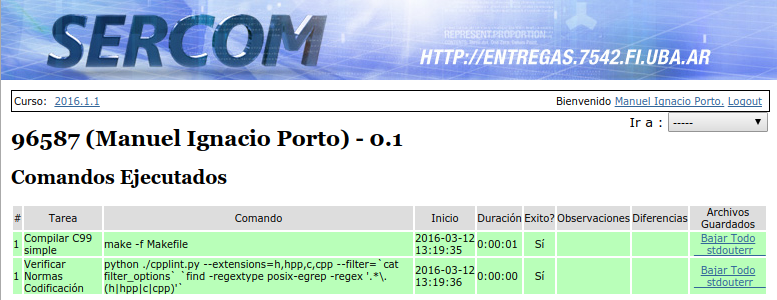
\includegraphics[width=\columnwidth]{p6_style}
        \caption{Chequeo de normas de codificación}
    \end{figure}
\textbf{Captura de pantalla con el resultado de la prueba 5}

    \begin{figure}[H]
        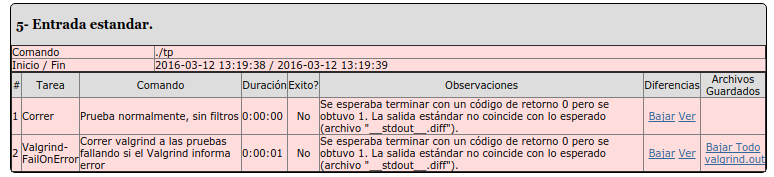
\includegraphics[width=\columnwidth]{p6_test5}
        \caption{Resultado de la prueba 5}
    \end{figure}

\section{SERCOM - Entrega exitosa}

\textbf{Captura de pantalla mostrando la entrega exitosa, en color verde.}
    \begin{figure}[H]
        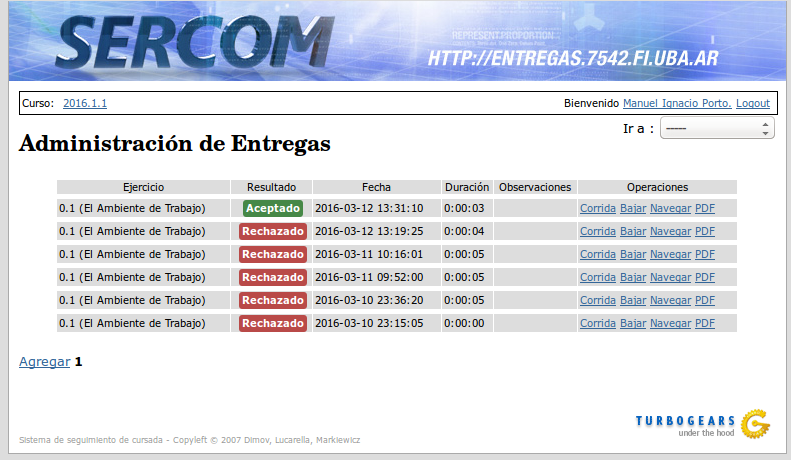
\includegraphics[width=\columnwidth]{p7_result}
        \caption{Entrega exitosa}
    \end{figure}
    
\textbf{Captura de pantalla mostrando la ejecución local de la prueba 5 sin el uso del teclado.}
    \begin{figure}[H]
        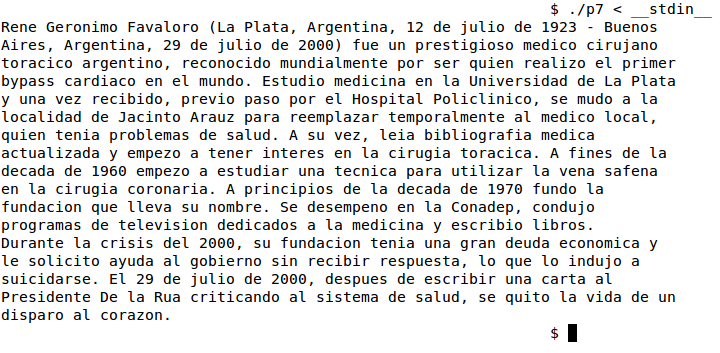
\includegraphics[width=\columnwidth]{p7_5}
        \caption{Entrega exitosa}
    \end{figure}
\textbf{Captura de pantalla mostrando la ejecución local de la prueba 2, pero redireccionando la salida
estándar a un archivo denominado ‘salida.txt’.}
    \begin{figure}[H]
        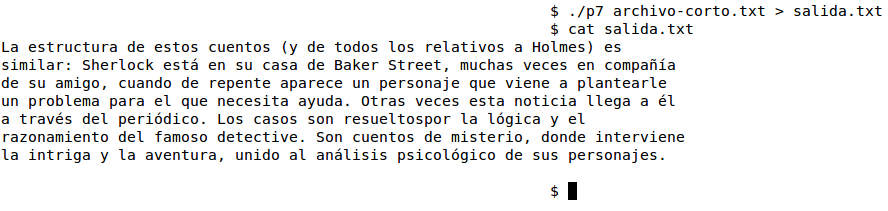
\includegraphics[width=\columnwidth]{p7_2}
        \caption{Entrega exitosa}
    \end{figure}
\end{document}
